\documentclass[aspectratio=169]{beamer}
\usetheme{Madrid}
\usecolortheme{default}

\usepackage{booktabs}
\usepackage{graphicx}
\usepackage{array}

\title[Pythia Repeat-Match Trajectory]{Pythia-14M Repeat-Match Checkpoint Trajectory}
\subtitle{Attention-role probes versus causal head ablation}
\author{Branch specialization research project}
\date{2026-05-22}

\begin{document}

\begin{frame}
  \titlepage
  \vspace{-0.5em}
  \small
  Checkpoint reason: this is the first real-transformer test of the
  probe-before-causality pattern found in the routed toy model.
\end{frame}

\begin{frame}{Question}
  The routed toy model showed:

  \vspace{0.5em}
  \begin{center}
  \textit{gate alignment can appear before causal branch modularity.}
  \end{center}

  \vspace{0.8em}
  Pythia has no router gate, so the real-model analogue is:

  \vspace{0.5em}
  \begin{center}
  \textit{does an attention-role probe appear before strong causal head
  importance?}
  \end{center}

  \vspace{0.8em}
  We test this on repeat-match heads across Pythia-14M training checkpoints.
\end{frame}

\begin{frame}{Setup}
  \begin{itemize}
    \item Models: \texttt{EleutherAI/pythia-14m-seed1}, seed2, seed3
    \item Revisions: step0, 64, 256, 1000, 4000, 16000, 64000, 143000
    \item Probe: attention from second occurrence of $x_i$ to first occurrence
    of $x_i$ in repeated-token sequences
    \item Causal test: zero selected head outputs and measure second-half
    next-token loss
    \item Heads tested: top repeat-match head in layers 0 and 1
    \item Controls: 8 random same-layer head sets per seed and checkpoint
  \end{itemize}

  \vspace{0.5em}
  Probe selection and causal evaluation use separate synthetic sequence sets.
\end{frame}

\begin{frame}{Metric Glossary}
  \begin{description}
    \item[Probe specialization] Normalized repeat-match attention score of the
    selected heads. This measures whether the head has the attention pattern.
    \item[Top loss delta] Loss after ablating selected repeat-match heads minus
    baseline loss.
    \item[Random loss delta] Same ablation metric for random same-layer heads.
    \item[Top minus random] Top-head loss delta minus random-head loss delta.
    This is the primary causal metric here.
  \end{description}

  \vspace{0.5em}
  The relative metric matters because some random head ablations improve this
  synthetic loss at intermediate checkpoints.
\end{frame}

\begin{frame}{Trajectory}
  \begin{center}
    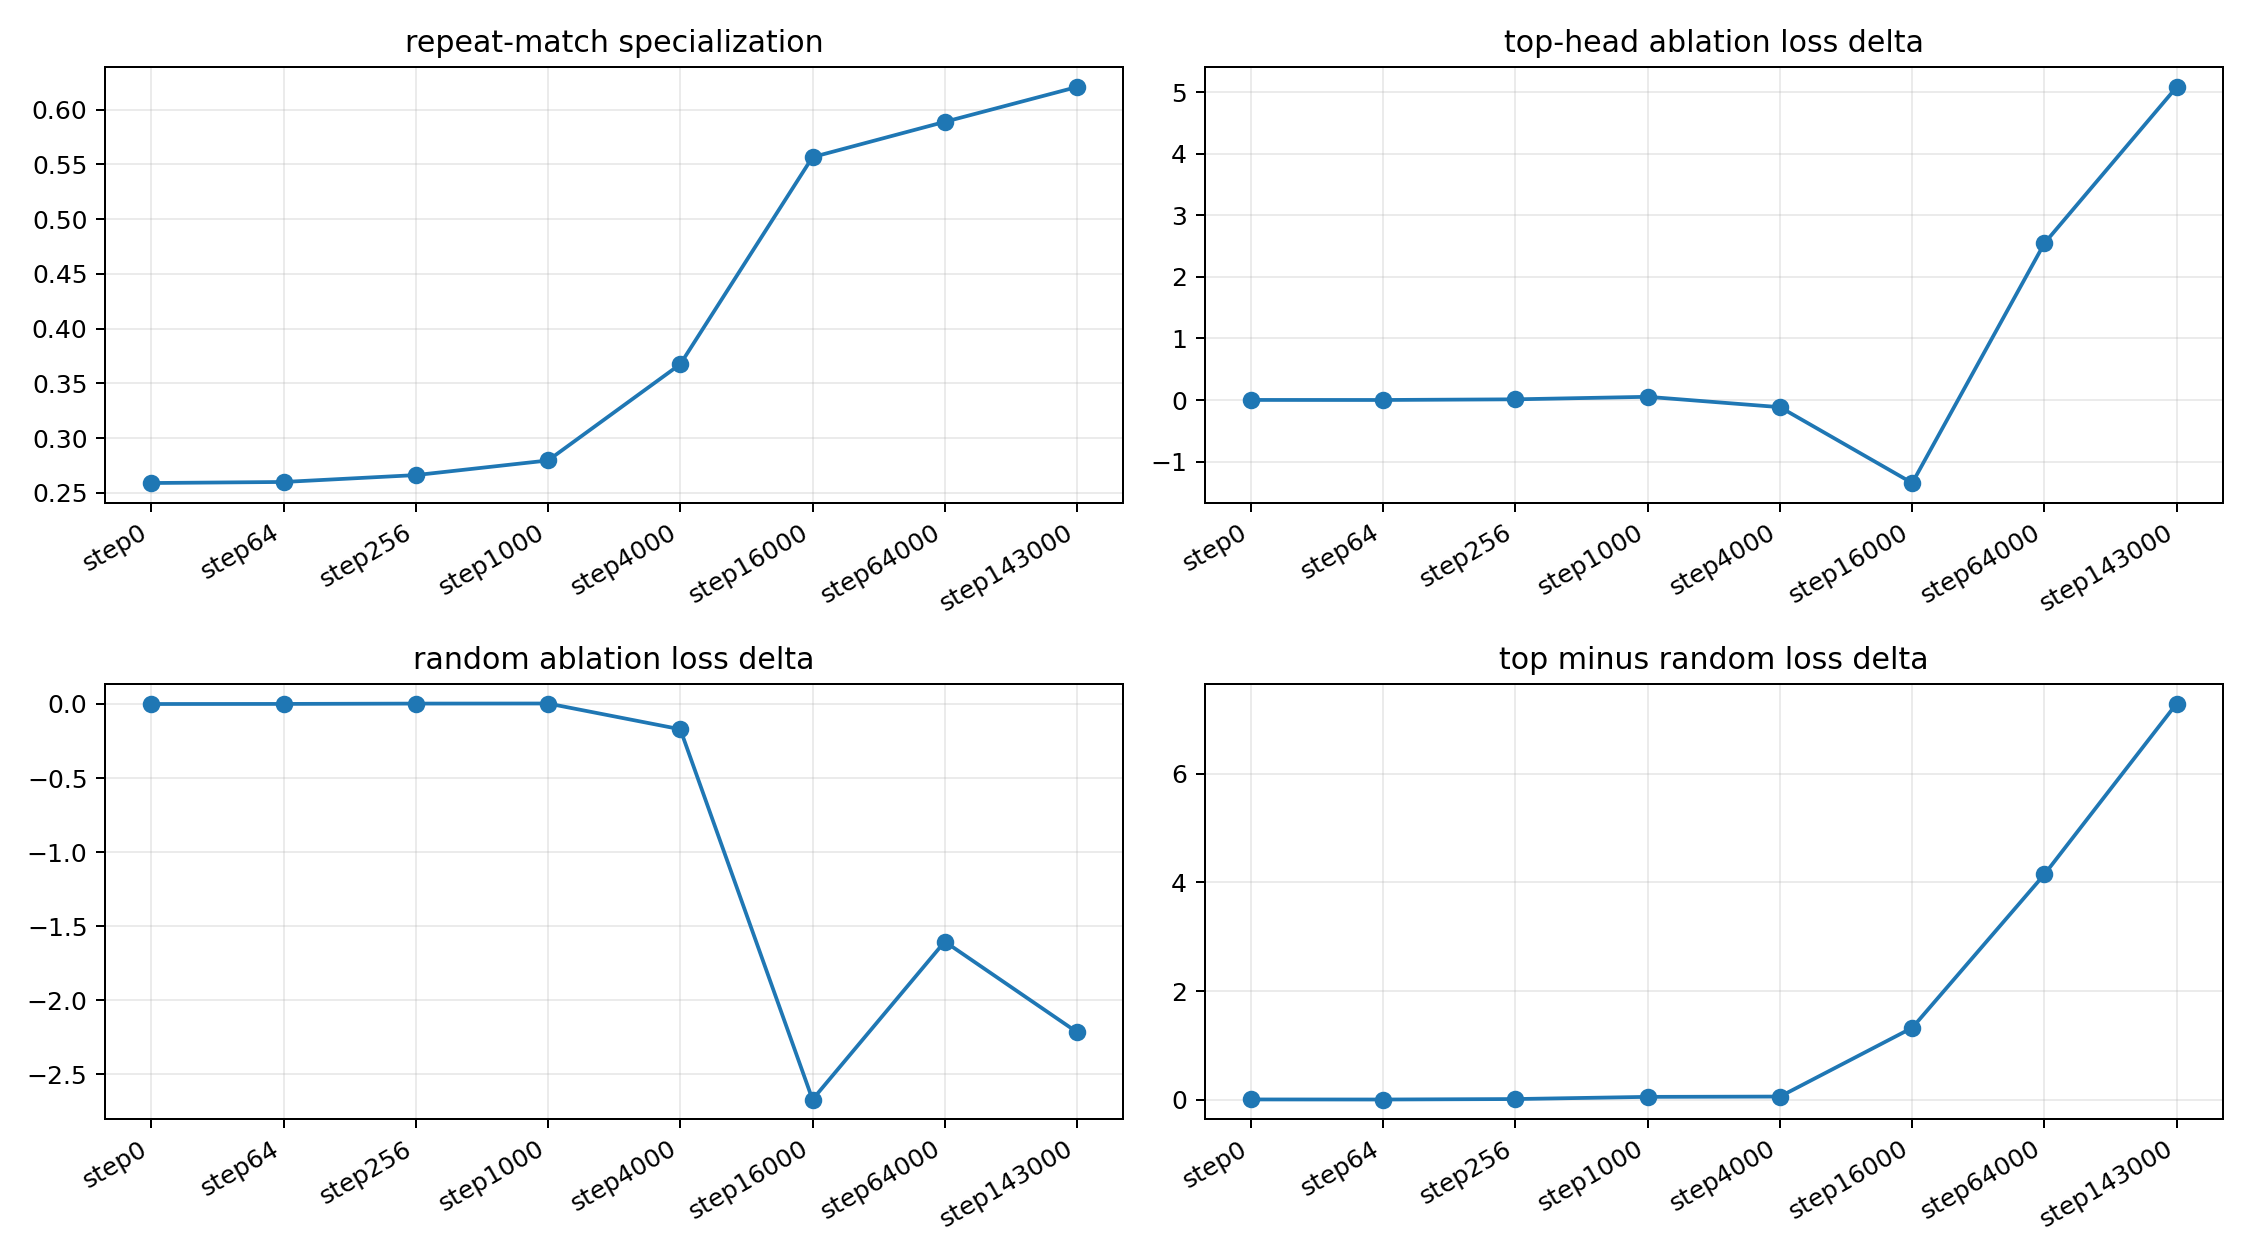
\includegraphics[height=0.70\textheight,keepaspectratio]{figures/repeat_match_checkpoint_trajectory.png}
  \end{center}

  \small
  Probe specialization starts rising before the top-minus-random causal excess
  becomes large. The causal excess is the bottom-right panel.
\end{frame}

\begin{frame}{Aggregate Results}
  \small
  \begin{center}
  \begin{tabular}{lrrrr}
    \toprule
    Revision & Probe spec. & Top loss & Random loss & Top $-$ random \\
    \midrule
    step0 & 0.2590 & 0.0018 & -0.0007 & 0.0025 \\
    step1000 & 0.2796 & 0.0527 & 0.0027 & 0.0500 \\
    step4000 & 0.3675 & -0.1155 & -0.1711 & 0.0556 \\
    step16000 & 0.5566 & -1.3471 & -2.6695 & 1.3224 \\
    step64000 & 0.5888 & 2.5466 & -1.6040 & 4.1506 \\
    step143000 & 0.6206 & 5.0833 & -2.2149 & 7.2982 \\
    \bottomrule
  \end{tabular}
  \end{center}

  \vspace{0.8em}
  Means over 3 seeds. The probe rises by step4000, while causal excess remains
  small until later checkpoints.
\end{frame}

\begin{frame}{Interpretation}
  \textbf{Supported}
  \begin{itemize}
    \item Repeat-match attention specialization can precede strong causal
    importance.
    \item This mirrors the toy result at the measurement level: probe/gate
    signals are not enough by themselves.
  \end{itemize}

  \vspace{0.7em}
  \textbf{Not shown}
  \begin{itemize}
    \item This does not show branch-level modularity in Pythia.
    \item These are ordinary attention heads, not routed branches.
  \end{itemize}
\end{frame}

\begin{frame}{Caveats}
  \begin{itemize}
    \item Pythia-14M pilot only; Pythia-160M remains the stronger target.
    \item 3 seeds only.
    \item Layers 0 and 1 only.
    \item Synthetic repeated-token task.
    \item Head-output ablation, not full path patching.
    \item Some random ablations improve synthetic loss, so use relative excess
    over random controls as the main causal readout.
  \end{itemize}
\end{frame}

\begin{frame}{Project-Level Update}
  The project now has the same methodological lesson in two settings:

  \begin{enumerate}
    \item Routed toy model: gate alignment preceded causal branch modularity.
    \item Pythia-14M: repeat-match specialization preceded strong causal head
    importance.
  \end{enumerate}

  \vspace{0.8em}
  The defensible paper framing is:

  \vspace{0.5em}
  \begin{center}
  \textit{specialization probes must be paired with causal tests, because the
  two can have different developmental timelines.}
  \end{center}
\end{frame}

\begin{frame}{Decision And Next Step}
  \textbf{Decision.} Keep the probe-versus-causality trajectory as a central
  measurement axis.

  \vspace{0.8em}
  \textbf{Next step.}
  Run the same checkpoint-trajectory analysis on Pythia-160M:
  \begin{itemize}
    \item use the already validated repeat-match layers;
    \item add cross-seed raw-score alignment;
    \item compare aligned transferred heads against same-index transferred heads
    across checkpoints.
  \end{itemize}
\end{frame}

\begin{frame}{Provenance}
  \small
  \textbf{Source}
  \begin{itemize}
    \item \texttt{scripts/pythia\_repeat\_match\_checkpoint\_trajectory.py}
    \item \texttt{doc/phase1\_pythia14m\_repeat\_match\_checkpoint\_trajectory.md}
  \end{itemize}

  \vspace{0.4em}
  \textbf{Copied data}
  \begin{itemize}
    \item \texttt{data/revision\_summary.csv}
    \item \texttt{data/revision\_seed\_summary.csv}
    \item \texttt{data/probe\_head\_scores.csv}
    \item \texttt{data/ablation\_results.csv}
    \item \texttt{figures/repeat\_match\_checkpoint\_trajectory.png}
  \end{itemize}

  \vspace{0.4em}
  \textbf{Run command}
  \begin{itemize}
    \item \texttt{python3 -u scripts/pythia\_repeat\_match\_checkpoint\_trajectory.py --model-size 14m --seeds 1 2 3 ...}
  \end{itemize}
\end{frame}

\end{document}
